\documentclass[12pt]{article} % For LaTeX2e
\usepackage{nips13submit_e,times}
\usepackage[colorlinks=true, urlcolor=blue]{hyperref}
\usepackage{url}
\usepackage{graphicx}
\usepackage{caption}
\usepackage{subcaption}
%\documentstyle[nips13submit_09,times,art10]{article} % For LaTeX 2.09


\title{CS 6675 Project Proposal (Group 17)\\Developing Fast, Scalable and Useful Recommendation System on Large Datasets}

\author{
Parminder Bhatia (Leader)\\
\And
Revant Kumar\\
\And
Gopi Krishnan Nambiar
}

% The \author macro works with any number of authors. There are two commands
% used to separate the names and addresses of multiple authors: \And and \AND.
%
% Using \And between authors leaves it to \LaTeX{} to determine where to break
% the lines. Using \AND forces a linebreak at that point. So, if \LaTeX{}
% puts 3 of 4 authors names on the first line, and the last on the second
% line, try using \AND instead of \And before the third author name.

\newcommand{\fix}{\marginpar{FIX}}
\newcommand{\new}{\marginpar{NEW}}

\nipsfinalcopy % Uncomment for camera-ready version

\begin{document}

\maketitle

\section{Motivation and Objectives}

Recommendations systems have become an integral cog in any business. Suggesting any product to the user that he/she might be interested in among the entire product catalog, helps  the user in saving time as well as makes the decision process easy. It also attracts the user in purchasing more, thus increasing the overall revenue for the company.

There has been a lot of research in building good recommender systems for the users. However, one of the biggest challenges is that of scalability, i.e. when the number of users and products are in the scale of millions. The objective of our project is to develop a scalable recommendation system, particularly Collaborative Filtering using the Map Reduce Paradigm. We also feel that social intuitions are really important for a good Collaborative Filtering algorithm, and thus we plan to also add social elements like location, number of friends etc. Adding Social elements can also help us in reducing the cold start problem, as we can get basic profile information about the person from demographics and other data from relevant social networks.

We plan to do optimized Matrix Factorization as a Map Reduce Task. We would also have to investigate as to how we can incorporate social elements so as provide decent results to new users.

\section{Related Work}

In [1], the authors have introduced a new idea to formulate topic based social influence analysis using Graph - (V,E) where V represented users or entities and E, for undirected edges.  The authors attempt to design a model which takes into consideration both topic distribution and network information to get a sense of the social influence, which is very different from the existing works on social network analysis conducted till that point of time. These two items are used as inputs for the program. In order to make the system conform to Map-Reduce framework, the authors implement a modified message passing algorithm which is compatible for the same. First, a Topic Factor Graph(TFG) is constructed which is a probabilistic model that includes all the information in a combined model. This is followed by the construction of the TAP model and parallelization procedure for the Map Reduce implementation. The TFG model consists of observed variables and latent variables as well which are the nodes in the network.
They have run the algorithm in a distributed manner which contributes to a speedup of about 15X for large datasets. As expected with parallel processing, this method is not efficient for smaller datasets.

[7] The cold-start recommendation task in an online retail setting for users who have not yet purchased (or interacted in a meaningful way with) any available items but who have granted access to limited side information, such as basic demographic data (gender, age, location) or social network information (Facebook friends or page likes). In this paper[7] ,  they formalize neighborhood-based methods for cold-start collaborative filtering in a generalized matrix algebra framework that does not require purchase data for target users when their side information is available. In real-data experiments with 30,000 users who purchased 80,000+ books and had 9,000,000+ Facebook friends and 6,000,000+ page likes, they show that using Facebook page likes for cold-start recommendation yields up to a 3-fold improvement in mean average precision (MAP) and up to 6-fold improvements in Precision and Recall compared to most-popular-item, demographic, and Facebook friend cold-start recommenders. These results demonstrate the substantial predictive power of social network content, and its significant utility in a challenging problem like recommendation for cold-start users.


\section{Proposed Method}

In order to build our recommendation system we will be using a class of algorithms called called collaborative filtering, specifically Item-Based Collaborative Filtering. The basic idea of collaborative filtering is very simple and intuitive. If a user has shown interest in item A and a second user has shown interest in A and B, then it's very likely that the first user may also be interested in item B. 

Now, we will explain the main parts of the project one by one:

\subsection{Data Collection}

In addition to item user data, we may have the user fill up a questionnaire, where he can select his interests, similar to what Quora, Pinterest do with the new user. We can also look into already build datasets such as MovieLens.

\subsection{User Engagement}

Level of user engagement can be estimated based on the following user actions. Typically, explicit rating by user is not available and other engagement events as below are used to estimate user's interest or engagement level.

\begin{itemize}
\item Time spent on a product page
\item Item added to wish list
\item Item added to shopping cart
\item Item purchased
\end{itemize}

\subsection{Utility Matrix}

All the social algorithms take an utility matrix as input. It contains data on user engagement for different items. In our case, If there are m items and n users, an utility matrix is a $m \times n$ matrix. The value of a matrix element $(i, j)$ represents the rating of an item $i$ by an user $j$. A row represents an item and it's associated ratings. A column represents an user and all the ratings for that user.

\begin{figure}[h]
\begin{center}
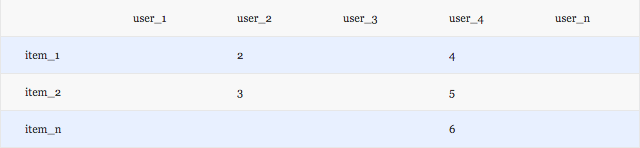
\includegraphics[width=5in]{user.png}
\end{center}
\end{figure}

The utility matrix is very sparse, because  typically a user will engage with a small fraction of the items available in the inventory. There is a duality about the utility matrix. The utility matrix can be used either to find similar items or similar users. We will be using item based similarity which has been found to produce better results.

\subsection{Algorithms for distance metric}

There are various social algorithms for distance metrics that can be used. We have listed some of them in the below table.

\begin{figure}[h]
\begin{center}
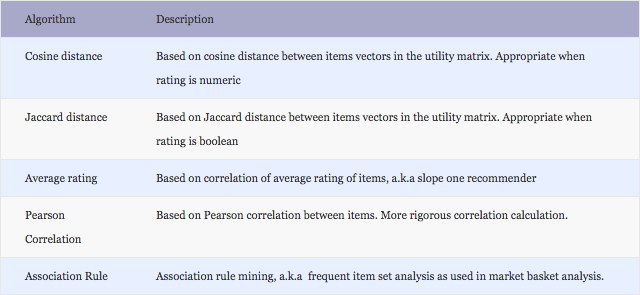
\includegraphics[width=5in]{measure.png}
\end{center}
\end{figure}

\subsection{Vector Distance}

Each row of the utility matrix represents an item. The values of the row vector are the ratings by different user. Essentially we find the cosine distance or jaccard between each pair of item vectors. Since these vector are sparse, they are effective means of finding similarities between the vectors.

\subsection{MapReduce/Hadoop/MRJOB}

MapReduce is a framework originally developed at Google that allows easy large scale distributed computing across a number of domains. Apache Hadoop is an open source implementation of it.  It scales well to many thousands of nodes and can handle petabytes of data. For recommendations where we have to find the similar products to a product you are interested at , we must calculate how similar pairs of items are. For instance, if someone watches the movie Matrix, the recommender would suggest the film Blade Runner. So we need to compute the similarity between two movies. One way is to find correlation between pairs of items.  But if you own a shopping site, which has 500,00 products, potentially we would have to compute over 250 billion computations. Besides the computation, the correlation data will be sparse, because it's unlikely that every pair of items will have some user interested in them. So we have a large and sparse dataset. And we have to also deal with temporal aspect since the user interest in products changes with time, so we need the correlation calculation done periodically so that the results are up to date.  For these reason the best way to handle with this problem is going after a divide and conquer pattern, and MapReduce is a powerful framework and can be used to implement data mining algorithms.

MRJob is a Python package that helps you write and run Hadoop Streaming jobs. It supports Amazon's Elastic MapReduce(EMR) and it also works with your own Hadoop cluster.  It has been released as an open-source framework by Yelp and we will use it as interface for Hadoop since it is easy to handle with MapReduce tasks.

\subsection{User Rating Support}

It may be desirable to exclude users who are not sufficiently engaged i.e the number of items that an user has been engaged with is below some percentage of the total number of items. This threshold is know as support in the data mining world. 

\subsection{Social Network Angle}

We know that humans are multifaceted. Only some of these facets are manifested in a social network. However, those facets may be relevant or irrelevant in the context of recommendation of some products and services. Thus, we will try to study whether an user's social network can be overlaid on the  utility matrix to create a personalized utility matrix, so that it could be used for recommendations.  Essentially, user's rating in the utility matrix could be weighted down by some radial function based on the degree separation in the social graph. 

\subsection{Flow Diagrams}

Flow diagrams can be seen in the Figures 1 and 2 above.

\begin{figure}
\centering
\begin{subfigure}{.5\textwidth}
  \centering
  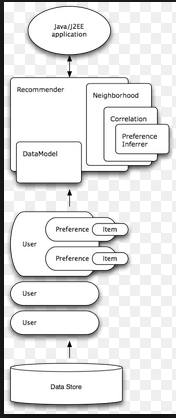
\includegraphics[width=0.7\linewidth]{flow1.jpg}
  \caption{Figure 1}
  \label{fig:sub1}
\end{subfigure}%
\begin{subfigure}{.5\textwidth}
  \centering
  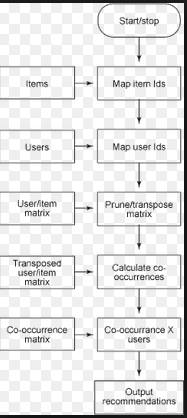
\includegraphics[width=0.75\linewidth]{flow2.jpg}
  \caption{Figure 2}
  \label{fig:sub2}
\end{subfigure}
\caption{Flow Diagrams}
\label{fig:test}
\end{figure}

\section{Plan of Action}

February:
\begin{itemize}
\item Week 2
	\begin{itemize}
	\item Preliminary preparation and setup
		\begin{itemize}
		\item Cluster setup
		\item Software stack familiarization
		\item Collection and decisions regarding the dataset, size and formatting
		\end{itemize}
	\item Testing and experimentation with algorithms on a local machine setup
	\end{itemize}
\item Week 3
	\begin{itemize}
	\item Data set finalization : Decide on test sets, training sets and on the final data source
	\end{itemize}
\item Week 4
	\begin{itemize}
	\item Perform experiments with CF on different parts of the dataset
		\begin{itemize}
		\item Experiment with the available algorithms
		\item Run the tests with the cleaned dataset on a Hadoop cluster
		\end{itemize}
	\item Data cleaning
	\end{itemize}
\end{itemize}

March:
\begin{itemize}
\item Week 1
	\begin{itemize}
	\item Algorithm improvements and tweaks
		\begin{itemize}
		\item Try to achieve improvements in the algorithms that already exist
		\end{itemize}
	\end{itemize}
\item Week 2, 3
	\begin{itemize}
	\item Application of algorithms
		\begin{itemize}
		\item Test with a suite of available tools and benchmark datasets to obtain efficient results for improvement of the recommender system
		\item These may be either applied from an open source library or a combination of libraries and manual techniques which are devised after significant experimentation with a  subset of the entire data available
		\end{itemize}
	\end{itemize}
\item Week 4
	\begin{itemize}
	\item Performance improvements
		\begin{itemize}
		\item Test and try to achieve performance improvements compared to the already existing algorithms.
		\end{itemize}
	\end{itemize}
\end{itemize}

April:
\begin{itemize}
\item Week 1,2
	\begin{itemize}
	\item Testing algorithms on the large dataset
		\begin{itemize}
		\item Polishing and fine tuning the algorithms for desired results
		\item Evaluation of the experiment results with current algorithms and techniques
		\end{itemize}
	\end{itemize}
\item Week 3,4
	\begin{itemize}
	\item Report
		\begin{itemize}
		\item A detailed report on the findings and improvements of this work over the current ones.
		\end{itemize}
	\end{itemize}
\end{itemize}

\section{Evaluation and Testing Method}

We will review and evaluate our recommender system using three types of experiments as follows:

\begin{enumerate}
\item Starting with an offline setting, where recommendation approaches are compared without user interaction
\item Then reviewing user studies, where a small group of subjects experiment with the system and report on the experience
\item Finally describe large scale online experiments, where real user populations interact with the system. 
\end{enumerate}

In each of these cases we plan to describe types of questions that can be answered, and suggest protocols for experimentation. We will also discuss how to draw trustworthy conclusions from the conducted experiments. We then review a large set of properties, and explain how to evaluate systems given relevant properties. We will also survey a large set of evaluation metrics in the context of the property that they evaluate.

Some Evaluation Metrics that we plan to report fall in two categories:

\begin{itemize}
\item Statistical Accuracy Metrics:
	\begin{itemize}
	\item Root Mean Square Error (RMSE)
	\item Mean Absolute Error (MAE)
	\item Correlation
	\end{itemize}
\item Decision Support Accuracy Metrics:
	\begin{itemize}
	\item Reversal Rates
	\item Weighted Errors
	\item ROC Sensitivity
	\end{itemize}
\end{itemize}

\section{Bibliography}
\begin{enumerate}
\item J. Tang, J. Sun, C. Wang, and Z. Yang. Social influence analysis in large-scale networks. In KDD, 2009.
\item User-based Collaborative-Filtering Recommendation Algorithms on Hadoop
\item http://aimotion.blogspot.com/2012/08/introduction-to-recommendations-with.html
\item https://pkghosh.wordpress.com/2012/04/21/socially-accepted-recommendation/
\item Guy Shani and Asela Gunawardana. Evaluating Recommendation System
\item Jonathan Herlocker, Joseph Konstan, Loren Terveen, and John Riedl. Evaluating Collaborative Filtering Recommender Systems. ACM Transactions on Information Systems, Vol. 22, No. 1, January 2004, Pages 5-53 
\item Social collaborative filtering for cold-start recommendations. S Sedhain, S Sanner, D Braziunas, L Xie - Proceedings of the 8th, 2014 - dl.acm.org 
\item Feng, Qinyuan, et al. "Enhancing personalized ranking quality through multidimensional modeling of inter-item competition." Collaborative Computing: Networking, Applications and Worksharing (CollaborateCom), 2010 6th International Conference on. IEEE, 2010.
\item Herlocker, Jonathan L., et al. "Evaluating collaborative filtering recommender systems." ACM Transactions on Information Systems (TOIS) 22.1 (2004): 5-53.
\end{enumerate}

\end{document}